\section{Roboterbau}

In diesem Teil werden die einzelne Schritte beschrieben, um den Roboter zu bauen. Dabei wird sich an dem Konzept auf \acrshort{pren1} orientiert. Falls von dem Konzept abgewichen wird, wird dies erwähnt und begründet. Die Arbeit aus \acrshort{pren1} kann im elektronischen Anhang gefunden werden.

Die folgenden Kapitel sind unterteilt nach den einzelnen Epics und User Stories, die im vorgehenden Kapitel \ref{projektplanung} aufgelistet wurden. Dabei werden die Tätigkeiten beschrieben, inklusive Testprotokolle und -beschriebe.

TODO: Risikoverweise (welches Risiko vermindert/behoben? Double check
with table from prev chapter 
TODO: Testprotokolle
TODO: Lessons Learned


%%%%%%%%%%%%%%%%%Epic 1%%%%%%%%%%%%%%%%%%%%%%%%%%%%%%%%%%%%%%%%%%%%%%%%%%%%%%%
\subsection{Fortbewegung mit geregelter Geschwindigkeit}

\subsubsection{Print Circuit Board design}
\label{pcb}

Um eine zuverlässige Kontaktierung der einzelnen Komponenten sicherzustellen, wird im Rah-
men von Pren 2 ein Verbindungs-PCB entwickelt. Dieses PCB übernimmt das Management der
Spannungsversorgung für den Raspberry Pi und den TinyK22. Zudem werden sämtliche Signale,
die vom TinyK22 erfasst und verarbeitet werden sollen, entsprechend verbunden.

Von dem PCB wurden fünf Exemplare bestellt. Ebenso sind von dem TinyK22 mehrere Exemplare vorhanden. Somit ist das Risiko der kaputten Elektroteile nicht mehr relevant. TODO IWAN: ANYTHING TO ADD?


\subsubsection{Motoren ansteueren und auslesen}

Nachdem die erste Ausführung der Software für die Motoren mit den beiden Encodern vorhanden war, wurde der implementierte Code mithilfe eines provisorischen Aufbaus getestet. Unter einem provisorischen Aufbau versteht man die Verwendung eines Breadboards mit dem TinyK22 und einem Speisegerät \ref{fig: Motorentest}. Allerdings wurde bereits der ausgewählte Motortreiber verwendet, der später auch im Endprodukt verbaut wird. Nach einigen Schwierigkeiten bei der Initialisierung des Quadratur-Encoder-Modus auf dem TinyK22 konnten die ersten Meter erfolgreich gefahren werden. Mit den ersten Erkenntnissen aus dem Test konnte die Software weiter angepasst werden, um immer präzisere Fahrmanöver auszuführen und die vorgegebenen Distanzen oder Drehwinkel exakt einzuhalten.


\begin{figure}[h]
\centering
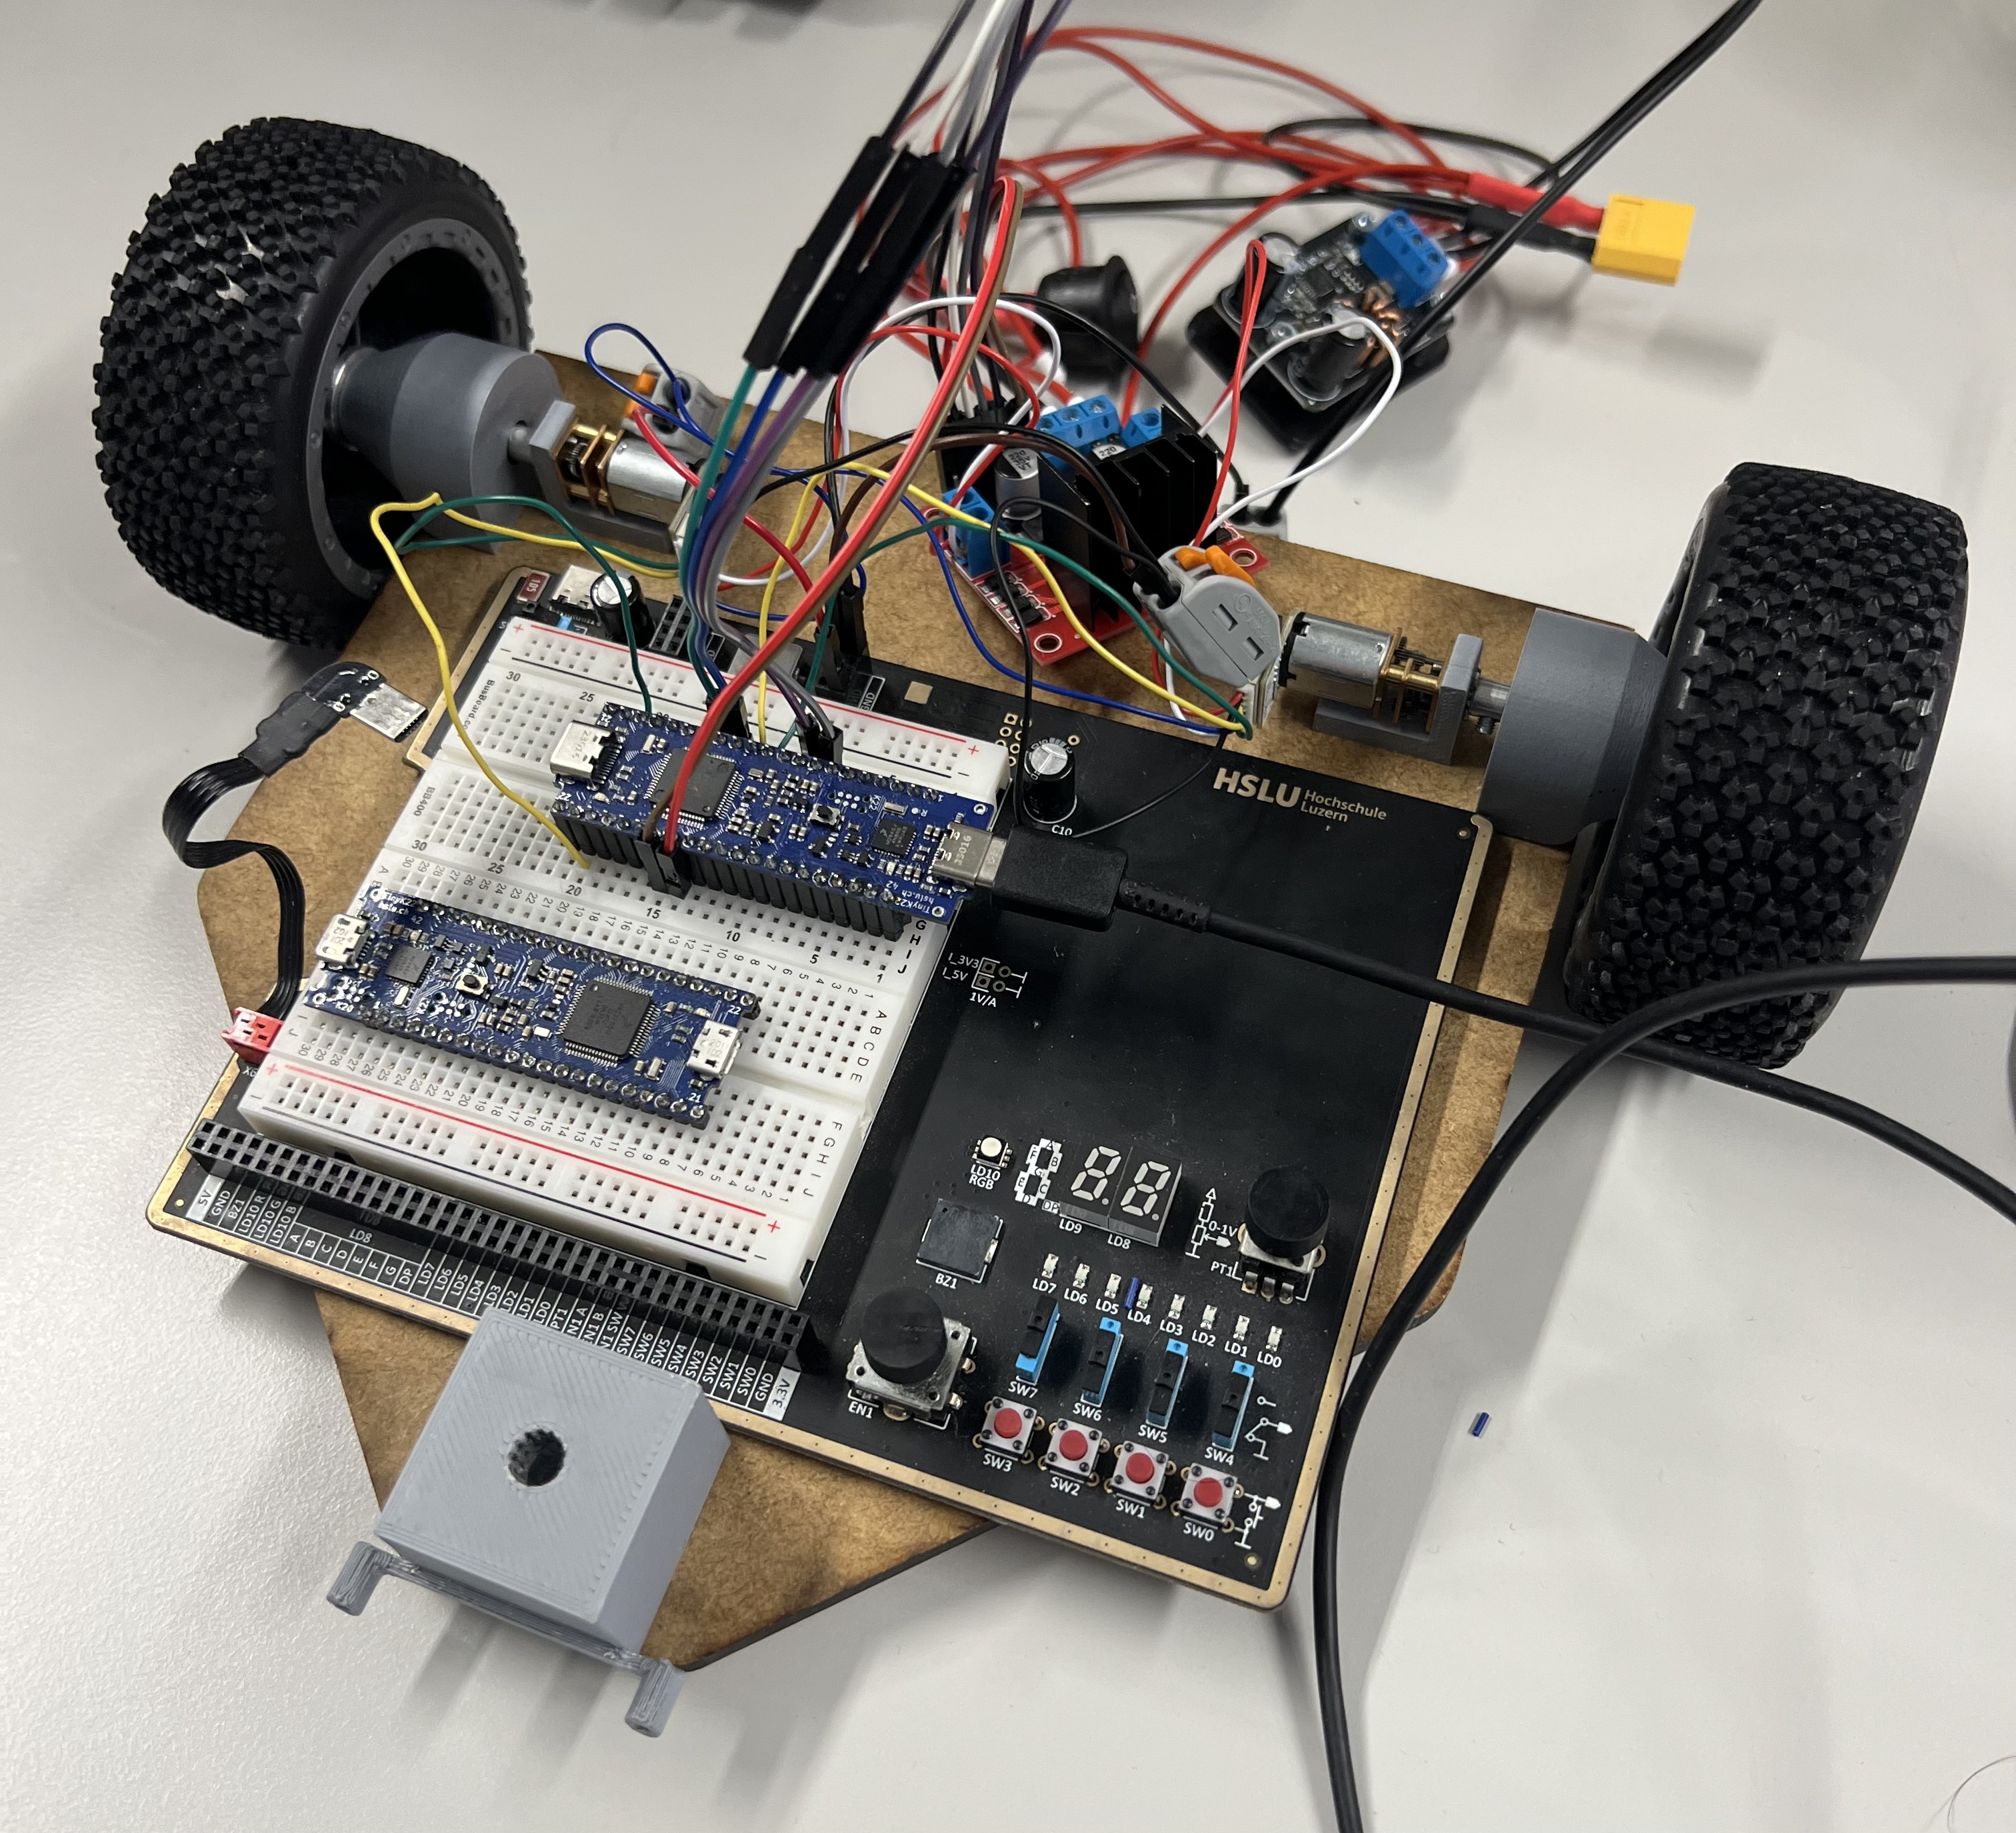
\includegraphics[width=10cm, height=8cm]{assets/ET/Motoren/Motorentest.jpeg}
\caption{Motorentest}
\label{fig: Motorentest}
\end{figure}

\subsubsection{Grundplatte konstruieren}

-Raeder, PCB, Tiny, Akku, Motoren


\newpage
%%%%%%%%%%%%%%%%%Epic 2%%%%%%%%%%%%%%%%%%%%%%%%%%%%%%%%%%%%%%%%%%%%%%%%%%%%%%%

\subsection{Auf Linien des Graphes bewegen}

\subsubsection{Liniensensor auslesen}

In einem ersten Durchlauf wurde ein Code implementiert, um die Funktion mit dem TinyK22 zu testen. Mittels eines Timers wurden die einzelnen Pins in einem genügend grossen Zeitabstand von Vcc auf Input Capture umgeschaltet. Nach dem Umschalten auf Input Capture sollten sich die Kondensatoren je nach Reflexion des Untergrunds in unterschiedlichen Zeiten entladen. Dieses Verhalten konnte im Testprogramm dann auch erfolgreich festgestellt werden, durch die unterschiedlichen Werten im Timer Register des Input Capture Modus.


TODO: schönes Bild vom Testgestell mit/für Liniensnesor

\subsubsection{Liniensensor mit Abschirmung anbringen}

Nach dem ersten Test wurde der Liniensensor am Fahrzeug angebracht. Um Störeinflüsse von aussen zu vermeiden, wurde eine Abdeckung konstruiert, die jegliche Einstrahlung abschirmt. Dank diesem Aufbau konnte mit der weiteren Implementierung begonnen werden. Für die Feineinstellung wurden die einzelnen Sensorwerte auf dem Originalboden ausgemessen – ebenso auf dem Klebeband, da dies essenziell ist, um die Regelung sauber abzustimmen.



TODO: schönes Bild vom Schlussgestell mit Abschirmung des Liniensensors


\newpage
%%%%%%%%%%%%%%%%%Epic 3%%%%%%%%%%%%%%%%%%%%%%%%%%%%%%%%%%%%%%%%%%%%%%%%%%%%%%%

\subsection{Bis zum nächsten Knoten fahren}

\subsubsection{Kameranbindung}

...

\subsubsection{Distanz berechnen}

...

\subsubsection{Liniensensor}

...